
\documentclass[12pt,a4paper]{report}

% -------------------- PACKAGES --------------------
\usepackage[utf8]{inputenc}
\usepackage[T1]{fontenc}
\usepackage{geometry}
\usepackage{graphicx}
\usepackage{float}
\usepackage{booktabs}
\usepackage{array}
\usepackage{longtable}
\usepackage{hyperref}
\usepackage{xcolor}
\usepackage{caption}
\usepackage{fancyhdr}
\usepackage{enumitem}
\usepackage{amsmath}
\usepackage{listings}

\geometry{margin=1in}
\setlength{\parskip}{6pt}
\setlength{\parindent}{0pt}
\setlength{\emergencystretch}{3em}

\hypersetup{
    colorlinks=true,
    linkcolor=blue,
    urlcolor=blue,
    citecolor=blue
}

\pagestyle{fancy}
\fancyhf{}
\lhead{Activity 2 -- Research Report}
\rhead{Department of MCA}
\cfoot{\thepage}

% -------------------- DOCUMENT --------------------
\begin{document}

% -------------------- TITLE PAGE --------------------
\begin{titlepage}
\centering

{\Large \textbf{JAIN (Deemed-to-be University)}}\\[0.3cm]
{\large Department of Computer Science and IT}\\[1.5cm]

{\Huge \textbf{ACTIVITY 2}}\\[0.4cm]
{\Large Student Research Report}\\[1.2cm]

\hrule
\vspace{0.5cm}

{\LARGE \textbf{NLP-Based Intelligent Writing Assistant: Autocorrect, Autocomplete, and POS-Aware Suggestions}}\\[0.4cm]
{\large Team Name: SyntaxSquad}

\vspace{0.5cm}
\hrule
\vspace{1cm}

\textbf{Submitted by}\\[0.3cm]

\begin{tabular}{ll}
Student 1: & Anoon M R (25MCAR0179) \\
Student 2: & Aman Kumawat (25MCAR0023) \\
Student 3: & Adithya Krishnan T N (25MCAR0003) \\
\end{tabular}

\vfill

\textbf{Course:} Natural Language Processing (25MCAAI303)\\
\textbf{Faculty:} Dr. Sharal Coelho\\
\textbf{Academic Year:} 2026--2027\\[0.5cm]

\textbf{Submission Date:} \underline{\hspace{4.5cm}}

\end{titlepage}

\pagenumbering{roman}
\tableofcontents
\clearpage
\pagenumbering{arabic}

% ==================================================
\chapter{Introduction}

\section{Background}

Writing assistance tools are among the most widely used applications of
Natural Language Processing, embedded in everyday software from mobile
keyboards to office suites and browsers. Most commercial tools, however,
operate as opaque black boxes built on proprietary, pre-trained models.
This project takes the opposite approach: every component -- spelling
correction, next-word prediction, and part-of-speech-aware filtering -- is
implemented from first principles in Python, directly applying the
statistical NLP techniques covered in Units 1 and 2 of this course (text
processing, edit distance, the noisy channel model, N-gram language
models, and Hidden Markov Model POS tagging with Viterbi decoding).

\section{Problem Statement}

Everyday digital writing is affected by three recurring issues that basic
tools handle poorly:
\begin{itemize}
    \item \textbf{Spelling errors} (typographical mistakes --
    insertions, deletions, substitutions, and transpositions) are often
    corrected without considering surrounding context or realistic error
    likelihoods.
    \item \textbf{Autocomplete suggestions} are frequently generated
    without regard to grammatical role, leading to suggestions that are
    statistically common but grammatically implausible in context (e.g.
    suggesting a noun where a verb is expected).
    \item \textbf{No lightweight, transparent, from-scratch NLP pipeline}
    was available that demonstrates how edit distance, the noisy channel
    model, N-gram language modeling, and HMM-based POS tagging work
    together as a single coherent system.
\end{itemize}

This project directly addresses all three by building each component from
first principles, without relying on pre-trained NLP libraries such as
NLTK's built-in taggers or spaCy models.

\section{Objectives}

\begin{enumerate}
    \item Implement a rule-based tokenizer for sentence and word
    segmentation.
    \item Implement a spelling corrector using the Noisy Channel Model,
    with Edit Distance candidate generation (up to two edits) and a
    channel model learned from a confusion matrix of real human
    misspellings.
    \item Implement bigram and trigram N-Gram Language Models with Laplace
    smoothing (trigram with back-off to bigram) for next-word prediction.
    \item Implement a bigram Hidden Markov Model POS tagger with Viterbi
    decoding, and use it to filter next-word suggestions by expected
    part of speech.
    \item Integrate all four components behind a live Flask web interface,
    and evaluate each component quantitatively on held-out data.
\end{enumerate}

\section{Scope of the Project}

The system operates entirely offline once the datasets are downloaded,
targets English text, and is trained on the Brown Corpus (via NLTK) plus
a corpus of real correct-word $\rightarrow$ misspelling pairs used to
learn the spelling channel model. The implementation covers the full
scope planned in the Phase~1 proposal:
\begin{itemize}
    \item spelling candidates at edit distance 1 \emph{and} 2;
    \item a channel model learned from deletion, insertion, substitution
    and transposition confusion matrices (Kernighan et al., 1990), not
    hand-chosen weights;
    \item bigram \emph{and} trigram language models, the trigram backing
    off to the bigram for unseen contexts;
    \item a live web interface that re-analyses the text as the user
    types, without reloading the page.
\end{itemize}
Remaining limitations (Laplace smoothing, a bigram HMM, and
isolated-word spelling correction) are discussed in
Chapter~\ref{ch:error} (Error Analysis).

% ==================================================
\chapter{Literature Survey}

\section{Comparison of Existing Research}

\small
\begin{longtable}{
|p{3.4cm}|p{2.6cm}|p{1.0cm}|p{3.2cm}|p{3.2cm}|
}
\caption{Comparative Analysis of Research Papers}\\
\hline
\textbf{Paper Title} &
\textbf{Publication} &
\textbf{Year} &
\textbf{Methodology} &
\textbf{Results / Findings} \\
\hline
\endfirsthead

\hline
\textbf{Paper Title} &
\textbf{Publication} &
\textbf{Year} &
\textbf{Methodology} &
\textbf{Results / Findings} \\
\hline
\endhead

A Technique for Computer Detection and Correction of Spelling Errors &
Communications of the ACM, 7(3) &
1964 &
Assumes a misspelled word has exactly one error (insertion, deletion,
substitution, or transposition) and searches a dictionary for the closest
match. &
Found that $\sim$80\% of real-world misspellings are single-error
misspellings; laid the groundwork for edit-distance-based correction
(Damerau--Levenshtein distance). \\
\hline

A Spelling Correction Program Based on a Noisy Channel Model &
COLING, Vol. 2, pp. 205--210 &
1990 &
Models a typo as the true word passed through a noisy channel; ranks
candidates by $P(\text{word}) \times P(\text{typo}\mid\text{word})$,
trained on AP newswire text. &
Established the noisy-channel formulation this project's spell corrector
is directly based on; channel probabilities learned from real confusion
data outperform frequency-only ranking. \\
\hline

Estimation of Probabilities from Sparse Data for the Language Model
Component of a Speech Recognizer &
IEEE Trans. Acoustics, Speech, and Signal Processing, ASP-35(3) &
1987 &
Proposes Katz back-off smoothing: unseen n-grams fall back to
lower-order n-gram estimates discounted via Good--Turing. &
More accurate than simple Laplace (add-one) smoothing on sparse n-gram
counts, directly motivating this project's planned Future Work
(Chapter~\ref{ch:conclusion}). \\
\hline

Class-Based n-gram Models of Natural Language &
Computational Linguistics, 18(4), pp. 467--480 &
1992 &
Clusters words into classes from co-occurrence statistics and builds
n-gram models over classes rather than individual words. &
Reduces data sparsity for n-gram prediction; relevant to scaling this
project's word-level bigram/trigram LM, whose trigram counts are very
sparse. \\
\hline

An Empirical Study of Smoothing Techniques for Language Modeling &
Computer Speech \& Language, 13(4), pp. 359--394 &
1999 &
Empirically compares Jelinek-Mercer, Katz, Witten-Bell, and Kneser-Ney
smoothing across corpus sizes and n-gram orders. &
Kneser-Ney (and a novel modified variant) consistently outperforms other
smoothing methods; directly explains why this project's
Laplace-smoothed models have high perplexity, and why the trigram's
is even higher than the bigram's (Chapter~\ref{ch:error}). \\
\hline

A Stochastic Parts Program and Noun Phrase Parser for Unrestricted Text &
2nd Conf. on Applied NLP (ANLP), pp. 136--143 &
1988 &
Uses dynamic programming (an HMM-style tagger) to balance lexical and
contextual tag probabilities, trained on the Brown Corpus. &
Reports 95--99\% tagging accuracy; this project's own HMM tagger (trained
on the same Brown Corpus) is directly comparable in design. \\
\hline

Error Bounds for Convolutional Codes and an Asymptotically Optimum
Decoding Algorithm &
IEEE Trans. Information Theory, 13(2), pp. 260--269 &
1967 &
Introduces the Viterbi algorithm: a dynamic-programming method for
finding the maximum-likelihood path through a trellis of states. &
The algorithm this project's POS tagger uses directly for exact
most-likely-tag-sequence decoding, originally developed outside NLP for
decoding convolutional codes. \\
\hline

TnT -- A Statistical Part-of-Speech Tagger &
6th Conf. on Applied NLP (ANLP-2000), pp. 224--231 &
2000 &
A trigram HMM tagger with careful smoothing and an explicit
unknown-word-handling model (suffix-based probability estimation). &
Shows a Markov-model (HMM) tagger can match or beat more complex
approaches such as Maximum Entropy; its unknown-word handling is a direct
source of inspiration for improving this project's current smoothing
(Chapter~\ref{ch:error}). \\
\hline

\end{longtable}
\normalsize

\section{Research Gap}

While the noisy channel model, n-gram smoothing, and HMM POS tagging are
each individually well studied (as shown above), the surveyed literature
largely treats them as separate problems solved in isolation, each
evaluated on its own benchmark. Few openly documented systems combine all
three into a single pipeline where POS tagging output directly filters
language-model suggestions in real time for an end user. This project
targets that integration gap: using the HMM tagger's transition
probabilities to filter the N-gram LM's next-word candidates
(Chapter~\ref{ch:methodology}, Section~\ref{sec:pos-filter}), rather than
running the two models independently.

% ==================================================
\chapter{Methodology}
\label{ch:methodology}

\section{Proposed Approach}

The system is implemented as a five-stage pipeline (Figure~\ref{fig:workflow}):
raw text is tokenized, spell-corrected, tagged for part of speech using an
HMM with Viterbi decoding, and the N-gram language model's next-word
candidates are then filtered by the POS tag the HMM expects to follow,
before being served to the user through a Flask web interface that
updates live as the user types.

\section{Dataset Description}

\begin{itemize}
    \item \textbf{Dataset name and source:} Brown Corpus, downloaded
    from the NLTK data repository (\url{https://www.nltk.org/nltk_data/})
    using NLTK's downloader, together with the Universal tagset mapping:
    \texttt{nltk.download('brown')} and
    \texttt{nltk.download('universal\_tagset')}. It is read through
    \texttt{nltk.corpus.brown} and was cleaned in Activity 1.
    \item \textbf{Number of samples:} 54,286 cleaned sentences (from
    57,340 raw sentences) for the language model; 54,270 POS-tagged
    sentences (Universal tagset) for the HMM tagger.
    \item \textbf{Vocabulary:} 24,891 words with frequency $\geq 2$
    (40,353 unique tokens total before filtering).
    \item \textbf{POS tag set:} 10 Universal tags -- ADJ, ADP, ADV, CONJ,
    DET, NOUN, NUM, PRON, PRT, VERB.
    \item \textbf{Misspelling corpus (channel model):}
    \texttt{spell-errors.txt} from Peter Norvig's \emph{Natural Language
    Corpus Data} \cite{norvig2009}, downloaded from
    \url{https://norvig.com/ngrams/spell-errors.txt}: 7,841 correct words, each listed with
    the ways real people misspelled it, giving 38,218
    (correct word, misspelling) pairs in total. This corpus is used to
    learn the spell corrector's confusion matrix and to test it on
    genuine human errors.
    \item \textbf{Preprocessing steps (Activity 1):} lowercasing,
    punctuation stripping, regex tokenization, filtering tokens shorter
    than 2 characters, and discarding sentences with fewer than 3 tokens.
\end{itemize}

\section{Algorithms and Technologies}

\begin{itemize}
    \item \textbf{Language:} Python 3.12
    \item \textbf{Web framework:} Flask 3.1.3
    \item \textbf{Tokenizer:} Regex-based sentence and word segmentation,
    preserving contractions (e.g. \texttt{isn't}).
    \item \textbf{Spell Corrector:} Noisy Channel Model
    \cite{kernighan1990}. For a misspelled word $x$, candidate corrections
    $c$ are all vocabulary words within edit distance 1 or 2 of $x$
    (insertion, deletion, substitution, transposition), ranked by
    \[
    \hat{c} = \arg\max_{c}\; P(c)\,P(x \mid c),
    \]
    where $P(c)$ is the Laplace-smoothed unigram prior from the Brown
    Corpus vocabulary and $P(x \mid c)$ is the channel probability. The
    channel model is learned: every single-edit (correct, misspelling)
    pair in the training split of the misspelling corpus is aligned to
    its one edit, which is counted in one of four confusion matrices
    (\texttt{del}, \texttt{ins}, \texttt{sub}, \texttt{trans}), keyed on
    the characters involved. For example,
    \[
    P(\text{del } y \text{ after } x) =
    \frac{\mathrm{del}[x,y] + 1}{\sum_{y'} \mathrm{del}[x,y'] + 26}.
    \]
    12,356 single-edit training pairs fill the matrices. For an
    edit-distance-2 candidate, the two edits' probabilities are
    multiplied.
    \item \textbf{N-Gram Language Model:} Bigram and trigram models,
    both with Laplace (add-one) smoothing:
    \[
    P(w_i \mid w_{i-1}) = \frac{C(w_{i-1}, w_i) + 1}{C(w_{i-1}) + V},
    \qquad
    P(w_i \mid w_{i-2}, w_{i-1}) =
    \frac{C(w_{i-2}, w_{i-1}, w_i) + 1}{C(w_{i-2}, w_{i-1}) + V},
    \]
    where $V$ is vocabulary size. If the two-word context
    $(w_{i-2}, w_{i-1})$ never occurred in training, the trigram
    backs off to the bigram estimate. Next-word prediction uses the
    trigram whenever two previous words are available.
    \item \textbf{HMM POS Tagger:} Bigram HMM with Laplace-smoothed
    transition ($A$), emission ($B$), and initial ($\pi$) probabilities,
    decoded with the Viterbi algorithm for exact most-likely tag
    sequences.
\end{itemize}

\section{POS-Aware Suggestion Filtering}
\label{sec:pos-filter}

After the HMM tags the corrected input, the tagger's transition matrix is
queried for $\arg\max_{t} P(t \mid \text{last\_tag})$ -- the POS tag most
likely to follow the current context. Each candidate word from the N-gram
model is independently assigned its own most-likely tag via
$P(\text{tag}\mid\text{word}) \propto P(\text{word}\mid\text{tag})\,P(\text{tag})$.
From the N-gram model's top 15 candidates, only those whose tag matches
the expected tag are kept, and the top 5 are shown. If no candidate
matches, the unfiltered list is shown instead, so the user always gets
suggestions. This is what distinguishes the system's suggestions from a
plain frequency-ranked autocomplete.

\section{System Workflow}

\begin{figure}[H]
\centering
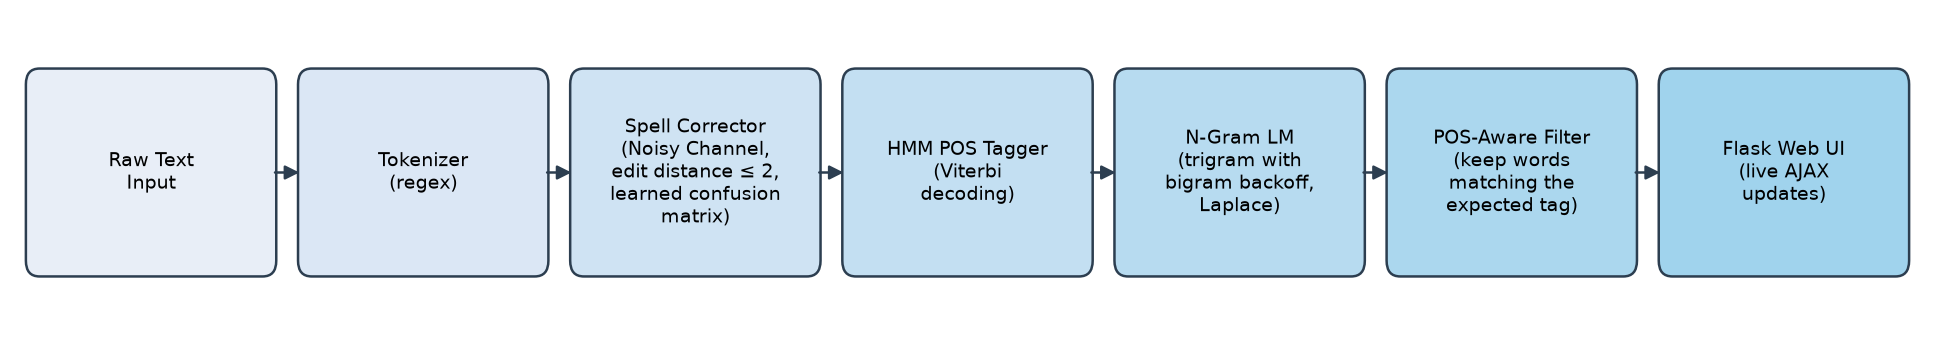
\includegraphics[width=0.95\textwidth]{assets/system_workflow.png}
\caption{Proposed System Workflow}
\label{fig:workflow}
\end{figure}

% ==================================================
\chapter{Experimental Details and Results}
\label{ch:results}

\section{Experimental Environment}

\begin{itemize}
    \item \textbf{Programming language:} Python 3.12
    \item \textbf{Development environment:} Claude Code CLI + local
    Python interpreter, Windows 11
    \item \textbf{Libraries and frameworks:} Flask 3.1.3, NLTK 3.8.1
    (Activity 1 only), matplotlib 3.11.1 (evaluation plots)
    \item \textbf{Hardware configuration:} Standard laptop CPU
    required -- all models are simple frequency/probability tables, not
    neural networks
    \item \textbf{Dataset split:} 90\% train / 10\% test, fixed random
    seed (42), applied independently to three datasets: the sentence set
    (48,858 train / 5,428 test, for the LM), the POS-tagged sentence set
    (for the HMM tagger), and the misspelling corpus (34,397 train /
    3,821 test pairs, for the spell corrector's confusion matrix). Every
    model is trained on its train split only and scored on its test split.
\end{itemize}

\section{Evaluation Metrics}

Five metrics were used across the three models:
\begin{itemize}
    \item \textbf{Spell Corrector (synthetic typos):} Top-1 correction
    accuracy on an auto-generated evaluation set of 200 sentences, each
    with exactly one induced edit-distance-1 typo (see
    Section~\ref{sec:evalset}).
    \item \textbf{Spell Corrector (real-world misspellings):} Top-1
    correction accuracy on 500 held-out (correct, misspelling) pairs
    from the misspelling corpus -- genuine human errors that the
    confusion matrix never saw during training.
    \item \textbf{N-Gram LM:} Bigram and trigram perplexity on the
    held-out 10\% test sentences --
    $\mathrm{PP} = \exp\!\left(-\frac{1}{N}\sum \ln P(w_i\mid \text{context})\right)$.
    \item \textbf{HMM POS Tagger:} Per-word tagging accuracy against gold
    Universal-tagset labels on 500 held-out test sentences.
\end{itemize}

\section{Evaluation Set Generation}
\label{sec:evalset}

Rather than hand-curating 200 test sentences, the evaluation set was
generated programmatically from held-out (test-split) Brown Corpus
sentences: for each sentence, one word was randomly selected and replaced
with a random edit-distance-1 variant (an insertion, deletion,
substitution, or transposition), simulating a realistic single-character
typo. This guarantees the ``correct answer'' for each typo is known
exactly, allowing automated accuracy scoring. The generated set is saved
as \texttt{report/evaluation\_set.json}.

\section{Experimental Results}

\begin{table}[H]
\centering
\caption{Performance of the Proposed System}
\begin{tabular}{|l|c|}
\hline
\textbf{Evaluation Metric} & \textbf{Obtained Value} \\
\hline
Spell Corrector top-1 accuracy (synthetic typos) & 76.00\% (152 / 200) \\
\hline
Spell Corrector top-1 accuracy (real-world misspellings) & 38.00\% (190 / 500) \\
\hline
N-Gram LM bigram perplexity (held-out) & 5595.97 \\
\hline
N-Gram LM trigram perplexity (held-out, with back-off) & 13641.36 \\
\hline
POS Tagger word accuracy (held-out) & 91.74\% (8242 / 8984) \\
\hline
\end{tabular}
\end{table}

All values are produced by \texttt{src/evaluate.py}, which saves them
to the file \texttt{report/evaluation\_results.json}. Re-running the
script reproduces them exactly, because the random seed is fixed.

\textbf{Spell corrector.} On synthetic single-edit typos the corrector
recovers the original word 76\% of the time. On genuine human
misspellings it scores 38\%, but this number has to be read alongside
how hard each misspelling is. Table~\ref{tab:realworld} breaks the 500
real test pairs down by their edit distance from the correct word.

\begin{table}[H]
\centering
\caption{Real-world spelling accuracy by edit distance}
\label{tab:realworld}
\begin{tabular}{|l|c|c|}
\hline
\textbf{Edit distance (correct $\rightarrow$ misspelling)} & \textbf{Pairs} & \textbf{Corrected} \\
\hline
1 & 173 & 112 (64.7\%) \\
\hline
2 & 134 & 78 (58.2\%) \\
\hline
3 or more & 193 & 0 (out of reach by design) \\
\hline
\textbf{Total} & \textbf{500} & \textbf{190 (38.0\%)} \\
\hline
\end{tabular}
\end{table}

193 of the 500 real misspellings (38.6\%) are three or more edits away
from the intended word, which a corrector that searches up to edit
distance 2 cannot reach. On the 307 misspellings that are within reach,
the corrector is right 61.9\% of the time (190 / 307).

\textbf{N-gram LM.} Both perplexities are high, and the trigram's is
higher than the bigram's. Both effects come from Laplace smoothing, not
from a counting error; Section~\ref{sec:smoothing-limitation} explains
why.

\textbf{POS tagger.} 91.74\% word-level accuracy with only Laplace
smoothing and no unknown-word model is a strong result for a
from-scratch bigram HMM trained on $\sim$49K sentences.

\section{Confusion Matrix}

The POS tagger is inherently a 10-class classification problem (one class
per Universal POS tag), so a confusion matrix was computed on the held-out
test set.

\begin{figure}[H]
\centering
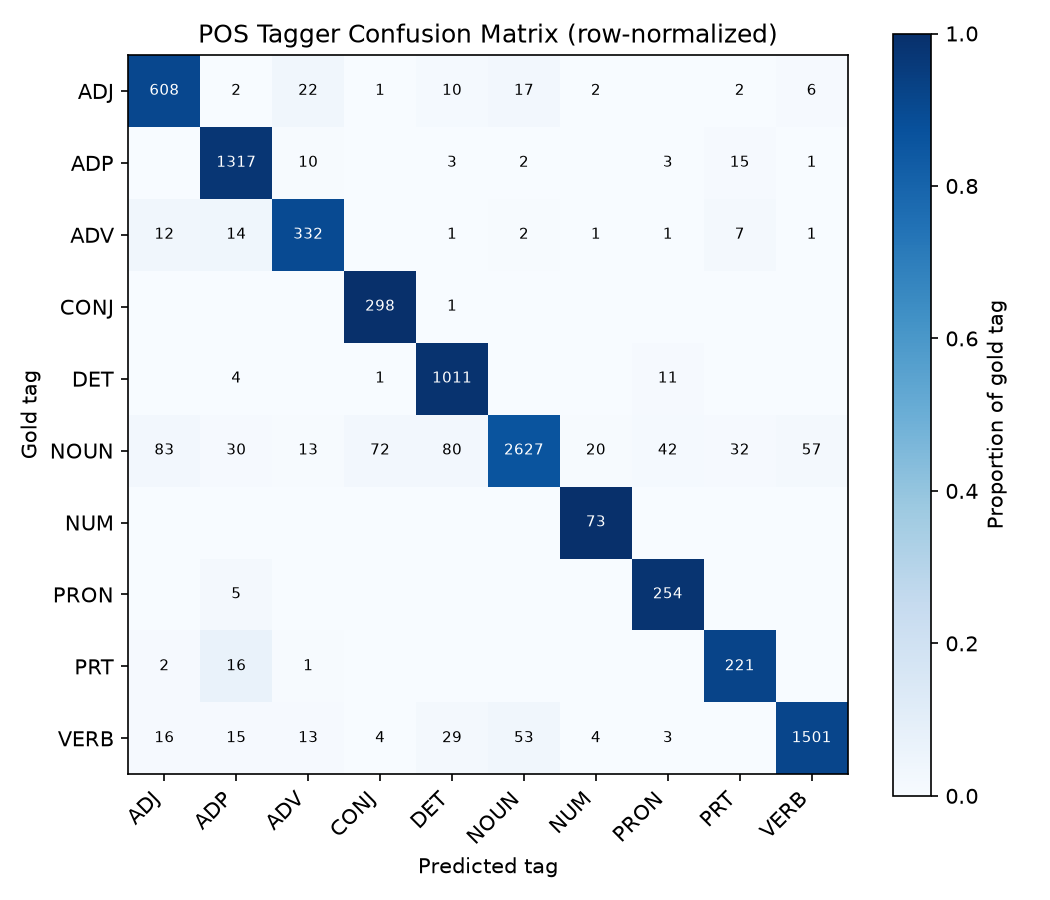
\includegraphics[width=0.78\textwidth]{assets/pos_confusion_matrix.png}
\caption{Confusion Matrix of the HMM POS Tagger (held-out test set, counts shown, color = row-normalized proportion)}
\label{fig:confusion}
\end{figure}

The matrix is strongly diagonal (correct predictions dominate every row).
The largest off-diagonal confusions are: NOUN misclassified as CONJ (72
instances) and ADJ (83 instances); and VERB/NOUN mutual confusion (53--57
instances each way). These are discussed in Chapter~\ref{ch:error}.

\section{Output Screenshots}

\begin{figure}[H]
\centering
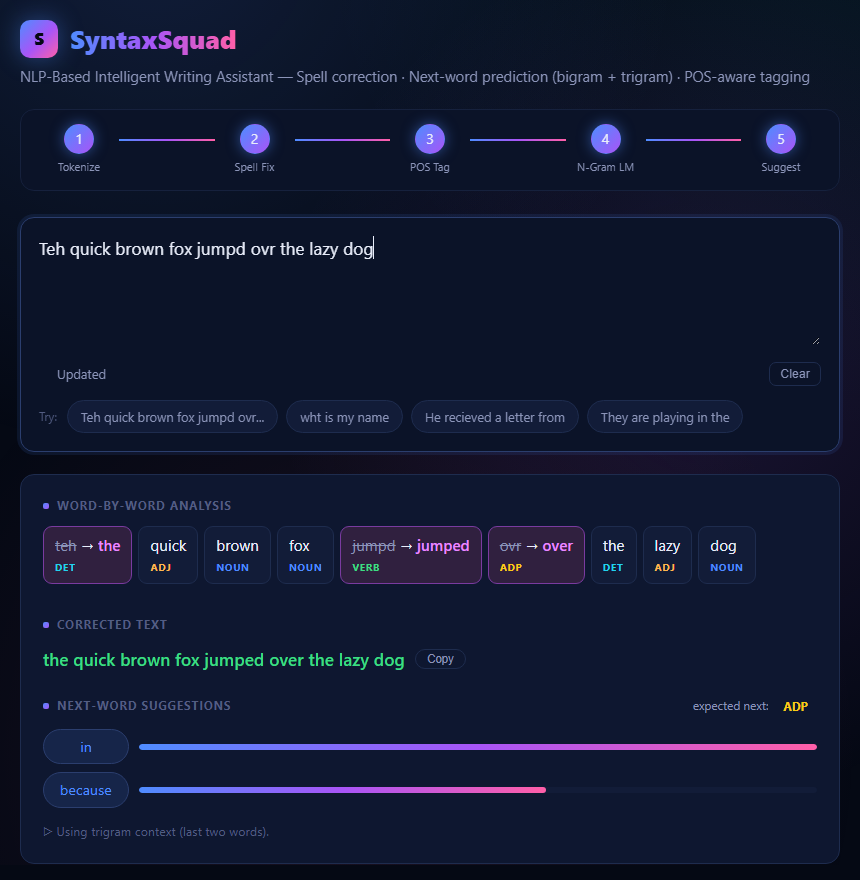
\includegraphics[width=0.85\textwidth]{assets/app_screenshot.png}
\caption{Live output of the Flask web app for the input ``Teh quick
brown fox jumpd ovr the lazy dog''. All three typos are fixed
(teh $\rightarrow$ the, jumpd $\rightarrow$ jumped, ovr $\rightarrow$
over; the strikethrough shows the original), every word is POS-tagged,
and the next-word suggestions (``in'', ``because'') are filtered to the
expected ADP tag using trigram context.}
\label{fig:output}
\end{figure}

% ==================================================
\chapter{Error Analysis}
\label{ch:error}

\section{Observed Errors}

\textbf{Spell Corrector -- why the 48 synthetic misses happened.} Each
of the 48 synthetic typos the corrector got wrong was inspected and
sorted into one of four groups (Table~\ref{tab:spellerrors}).

\begin{table}[H]
\centering
\caption{Breakdown of the 48 synthetic-typo misses}
\label{tab:spellerrors}
\begin{tabular}{|>{\raggedright\arraybackslash}p{6.2cm}|c|>{\raggedright\arraybackslash}p{5cm}|}
\hline
\textbf{Cause} & \textbf{Count} & \textbf{Example (intended $\rightarrow$ typo $\rightarrow$ output)} \\
\hline
A very frequent word two edits away beat the correct word one edit away & 23 &
head $\rightarrow$ haed $\rightarrow$ \emph{and}; source $\rightarrow$ sourhe $\rightarrow$ \emph{course} \\
\hline
A different one-edit word with a higher score won & 11 &
here $\rightarrow$ herp $\rightarrow$ \emph{help} \\
\hline
The typo is itself a real word, so it is never flagged & 9 &
will $\rightarrow$ gill; the $\rightarrow$ she \\
\hline
The intended word is not in the vocabulary & 5 &
silkworms $\rightarrow$ xsilkworms \\
\hline
\end{tabular}
\end{table}

The largest group (23 of 48) is a side effect of extending the search to
edit distance 2: the unigram prior of a very common word such as
``and'' is large enough to outweigh the extra edit's channel penalty.
This is also the main reason synthetic-typo accuracy fell from 85.5\%
in the earlier, edit-distance-1-only version of the system to 76\% now.
The trade is deliberate: edit distance 2 is what makes 78 of the
real-world misspellings in Table~\ref{tab:realworld} correctable at
all, and the learned confusion matrix fixed specific failures of the
earlier version, such as ``ovr'' $\rightarrow$ ``or'' (now ``over'')
and ``wht'' $\rightarrow$ ``who'' (now ``what'').

\textbf{Spell Corrector -- out-of-reach real misspellings.} 193 of the
500 real-world test misspellings are three or more edits from the
intended word (Table~\ref{tab:realworld}); some are not typos at all
but phonetic or alternate spellings. None of these can be corrected by
an edit-distance-2 search.

\textbf{POS Tagger -- NOUN confusions.} The largest off-diagonal cells
in Figure~\ref{fig:confusion} are NOUN predicted as ADJ (83), DET (80)
and CONJ (72), plus mutual NOUN/VERB confusion (53--57 each way). These
are concentrated on lexically ambiguous words (e.g.\ ``that'') where
the bigram HMM's one-tag context window cannot fully disambiguate.

\textbf{N-Gram LM -- high perplexity, and trigram higher than bigram.}
Bigram perplexity is 5,596 and trigram perplexity is 13,641 on held-out
data.

\section{Possible Causes}

\begin{itemize}
    \item The spell corrector scores candidates at edit distance 1 and 2
    on equal terms, apart from the channel probability. It has no
    explicit preference for fewer edits, so a high enough prior lets a
    two-edit word win.
    \item The corrector looks at each word in isolation, so a typo that
    happens to form another real word (``gill'' for ``will'') is never
    flagged. Catching these needs the sentence context (a real-word
    error model).
    \item The confusion matrix is sparse: 12,356 single-edit training
    pairs spread over roughly 2,700 possible (character, edit)
    combinations, so many specific edits have only a handful of counts.
    \item The HMM tagger's bigram context (only the immediately preceding
    tag) is a known limitation relative to trigram HMMs such as TnT
    (Brants, 2000, surveyed in Chapter 2).
    \item \label{sec:smoothing-limitation} Laplace smoothing adds the
    full vocabulary size $V \approx 40{,}000$ to every denominator,
    regardless of how often the context occurred (Chen \& Goodman, 1999).
    Trigram contexts are far rarer than bigram contexts, so for a
    typical trigram context $C(w_{i-2}, w_{i-1})$ is tiny compared with
    $V$, and almost all the probability mass is spread uniformly over
    unseen words. That is why the trigram's perplexity is higher than
    the bigram's, even though a trigram has more context: the problem
    is the smoothing, not the extra context.
\end{itemize}

\section{Improvement Strategies}

\textbf{Implemented in the current system:}
\begin{itemize}
    \item A learned confusion matrix replaced the earlier fixed
    per-edit-type weights. This fixed the ``ovr'' $\rightarrow$ ``or''
    and ``wht'' $\rightarrow$ ``who'' errors found during manual testing.
    \item Spelling candidates were extended to edit distance 2, making 78
    real-world misspellings correctable that were previously out of reach.
    \item The trigram model backs off to the bigram for unseen contexts,
    so suggestions never collapse to a uniform guess.
    \item Single-letter words (``I'', ``a''), which Activity 1's
    preprocessing excluded from the vocabulary, are special-cased as
    known words after ``I'' was being ``corrected'' to ``in'' during
    testing.
    \item The POS-aware suggestion filter (Section~\ref{sec:pos-filter})
    was added after testing showed that plain frequency-ranked
    suggestions ignored grammatical role.
\end{itemize}

\textbf{Suggested for future work (not yet implemented):}
\begin{itemize}
    \item Prefer edit-distance-1 candidates whenever one exists (or
    apply an explicit penalty per extra edit). This directly targets
    the largest group of synthetic misses.
    \item Use the language model to rank spelling candidates in context,
    which would also catch real-word errors such as ``gill'' for
    ``will''.
    \item Replace Laplace smoothing with Katz back-off or Kneser-Ney
    smoothing to reduce perplexity, especially for the trigram.
    \item Extend the HMM to a trigram model for richer context,
    following the TnT tagger's design.
\end{itemize}

% ==================================================
\chapter{Project Proof and Implementation Evidence}

\section{GitHub Repository}

\textbf{Repository URL:}
\url{https://github.com/AnoonMR/Writing-Assistant}

The repository contains the complete Activity 2 project: the source code
for all five modules, the evaluation script, the preprocessed datasets,
the README with setup instructions, and this report with its
presentation. The Activity 1 dataset download and preprocessing scripts
are in a separate repository, \url{https://github.com/AnoonMR/nlp-a1}.

\section{Deployment Evidence}

\textbf{Deployment:} Not deployed to a public hosting service. The
application is designed to run locally: all datasets are downloaded once
(Activity 1), after which the entire system -- language model, spell
corrector, POS tagger, and Flask server -- runs fully offline on
\texttt{localhost}. This was a deliberate scope decision for a course
mini-project rather than a limitation of the architecture; nothing in the
design prevents deploying it to a hosting service such as Render or
PythonAnywhere if required.

To run locally:
\begin{enumerate}
    \item \texttt{pip install -r requirements.txt}
    \item \texttt{cd src}, then \texttt{python app.py}
    \item Open \url{http://127.0.0.1:5000} in a browser and start typing;
    results update live, with no button to press.
\end{enumerate}

To reproduce every number in Chapter~\ref{ch:results}, run
\texttt{python evaluate.py} from the same \texttt{src} folder.

\section{Deployed Application Screenshot}

See Figure~\ref{fig:output} (Chapter~\ref{ch:results}), which shows the
live local application running and producing real output.

% ==================================================
\chapter{Conclusion and Future Work}
\label{ch:conclusion}

\section{Conclusion}

This project implemented a complete, from-scratch NLP pipeline for an
intelligent writing assistant, covering all five planned modules:
tokenizer, Noisy Channel spell corrector with a learned confusion matrix,
bigram and trigram N-gram language models, HMM POS tagger with Viterbi
decoding, and a live Flask web interface that ties them together with
POS-aware suggestion filtering. All objectives stated in Chapter 1 were
achieved, at the full scope planned in the Phase~1 proposal.

Quantitatively, on held-out data the system reaches 91.74\% POS-tagging
accuracy and 76\% top-1 spelling accuracy on synthetic typos. On genuine
human misspellings it reaches 38\% overall, rising to 61.9\% on the
misspellings within its edit-distance-2 search range. These are models
trained entirely from first principles (no pre-trained taggers or
embeddings) on a single mid-sized corpus. Every weak point found -- the
frequency bias of edit-distance-2 candidates, out-of-range misspellings,
and the high perplexity caused by Laplace smoothing -- has a measured,
explained cause (Chapter~\ref{ch:error}) and a concrete fix.

\section{Future Work}

\begin{itemize}
    \item Prefer edit-distance-1 spelling candidates when one exists, or
    penalise each extra edit, to remove the largest group of spelling
    errors.
    \item Rank spelling candidates using the language model in context,
    which would also catch real-word errors.
    \item Replace Laplace smoothing with Katz back-off or Kneser-Ney
    smoothing, which should lower perplexity, especially for the trigram.
    \item Extend the HMM tagger to trigram context.
    \item Optionally deploy the Flask app to a public hosting service.
\end{itemize}

% ==================================================
\chapter{Acknowledgement of AI Usage}

\section{AI Usage Statement}

This project was developed with the assistance of Claude (Anthropic), an
AI tool, which was used for code implementation and debugging.

% ==================================================
\begin{thebibliography}{99}

\bibitem{damerau1964}
F. J. Damerau, ``A technique for computer detection and correction of
spelling errors,''
\textit{Communications of the ACM}, vol. 7, no. 3, pp. 171--176, 1964.
DOI: 10.1145/363958.363994.

\bibitem{kernighan1990}
M. D. Kernighan, K. W. Church, and W. A. Gale, ``A spelling correction
program based on a noisy channel model,''
\textit{Proceedings of COLING}, vol. 2, pp. 205--210, 1990.

\bibitem{katz1987}
S. M. Katz, ``Estimation of probabilities from sparse data for the
language model component of a speech recognizer,''
\textit{IEEE Transactions on Acoustics, Speech, and Signal Processing},
vol. ASP-35, no. 3, pp. 400--401, 1987.

\bibitem{brown1992}
P. F. Brown, V. J. Della Pietra, P. V. deSouza, J. C. Lai, and R. L.
Mercer, ``Class-based n-gram models of natural language,''
\textit{Computational Linguistics}, vol. 18, no. 4, pp. 467--480, 1992.

\bibitem{chen1999}
S. F. Chen and J. Goodman, ``An empirical study of smoothing techniques
for language modeling,''
\textit{Computer Speech \& Language}, vol. 13, no. 4, pp. 359--394, 1999.

\bibitem{church1988}
K. W. Church, ``A stochastic parts program and noun phrase parser for
unrestricted text,''
\textit{Proceedings of the 2nd Conference on Applied Natural Language
Processing (ANLP)}, pp. 136--143, 1988. DOI: 10.3115/974235.974260.

\bibitem{viterbi1967}
A. J. Viterbi, ``Error bounds for convolutional codes and an
asymptotically optimum decoding algorithm,''
\textit{IEEE Transactions on Information Theory}, vol. 13, no. 2,
pp. 260--269, 1967.

\bibitem{norvig2009}
P. Norvig, ``Natural language corpus data,'' in \textit{Beautiful Data},
T. Segaran and J. Hammerbacher, Eds. O'Reilly Media, 2009, pp. 219--242.
Data: \url{https://norvig.com/ngrams/}.

\bibitem{brants2000}
T. Brants, ``TnT -- A statistical part-of-speech tagger,''
\textit{Proceedings of the 6th Conference on Applied Natural Language
Processing (ANLP)}, pp. 224--231, 2000. DOI: 10.3115/974147.974178.

\end{thebibliography}

\end{document}
